% Preamble
\documentclass[../Relazione_circuiti]{subfiles}
% \usepackage{amstex} Mi si era aggiunto da solo, magari un giorno capiamo che serve

% Packages
\graphicspath{{\subfix{../images/}}}

% Document
\begin{document}

Questo esperimento vuole verificare la validità delle formule teoriche su un filtro crossover reale.

\begin{wrapfigure}{r}{6.6cm}
  \centering
  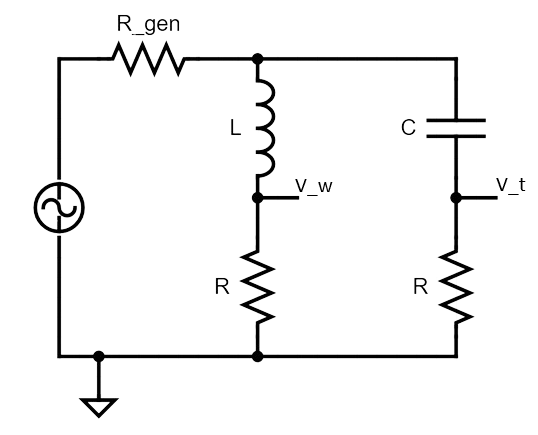
\includegraphics[width=6cm]{Schema_crossover.png}
  \caption{Schema del circuito realizzato}
  \label{fig:schema_circuito}
\end{wrapfigure}

Il filtro crossover è un circuito RLC costituito da due rami: uno con un filtro passa basso realizzato mediante un
induttore (ramo \textbf{Woofer}), l'altro con un filtro passa alto costituito da un condensatore (ramo
\textbf{Tweeter}).
Le due resistenze (tal volta dette \textit{resistenze di carico}) nella Fig.\,\ref{fig:schema_circuito} simulano degli
altoparlanti (da qui i nomi dei rami), e sono da considerarsi uguali a meno delle incertezze.

Le componenti di un segnale oscillante in ingresso, vengono scalate in ampiezza sui rami del circuito in base alla loro
frequenza.
Il ramo del \textit{woofer} presenta un'attenuazione progressiva delle componenti ad alta frequenza, mentre il ramo
del \textit{tweeter} di quelle a bassa.
La frequenza alla quale un segnale è ripartito in egual modo sui due rami è detta \textit{frequenza di cross} e dipende
dai valori della capacità e dell'induttanza del circuito.
Per calcolarla basta eguagliare le impedenze dei due rami, e si ottiene facilmente:
\begin{equation}
  \label{eq:f_cross}
  \nu_{cross} = \frac{1}{2 \pi \sqrt{LC} }
\end{equation}
dove $L$ è l'induttanza della bobina sul ramo Woofer e $C$ la capacità del condensatore sul ramo del Tweeter.

Le impedenze dei rami introducono anche uno sfasamento rispetto al generatore:
\begin{equation}
\label{eq: p_w_t}
  \phi_{woofer}(\omega) = \arctan(-\frac{\omega L}{R}) \qquad \quad %\label{eq:p_woofer}
  \phi_{tweeter}(\omega) = \arctan(\frac{1}{\omega RC}) %\label{eq:p_tweeter}
\end{equation}
dove $\omega$ è la pulsazione dell'onda in ingresso e $R$ il valore delle resistenze sui due rami.
Inoltre per la differenza di fase relativa si ha:
\begin{equation}
  \label{eq:p_diff}
  \Delta \phi(\omega) = \phi_{tweeter}(\omega) - \phi_{woofer}(\omega) = \arctan(\frac{1}{\omega RC}) + \arctan(\frac{\omega L}{R})
\end{equation}



\end{document}